%%% The main file. It contains definitions of basic parameters and includes all other parts.

%% Settings for single-side (simplex) printing
% Margins: left 40mm, right 25mm, top and bottom 25mm
% (but beware, LaTeX adds 1in implicitly)
\documentclass[12pt,a4paper]{report}
\setlength\textwidth{145mm}
\setlength\textheight{247mm}
\setlength\oddsidemargin{15mm}
\setlength\evensidemargin{15mm}
\setlength\topmargin{0mm}
\setlength\headsep{0mm}
\setlength\headheight{0mm}
% \openright makes the following text appear on a right-hand page
\let\openright=\clearpage

%% Settings for two-sided (duplex) printing
% \documentclass[12pt,a4paper,twoside,openright]{report}
% \setlength\textwidth{145mm}
% \setlength\textheight{247mm}
% \setlength\oddsidemargin{14.2mm}
% \setlength\evensidemargin{0mm}
% \setlength\topmargin{0mm}
% \setlength\headsep{0mm}
% \setlength\headheight{0mm}
% \let\openright=\cleardoublepage

%% Generate PDF/A-2u
\usepackage[a-2u]{pdfx}

%% Character encoding: usually latin2, cp1250 or utf8:
\usepackage[utf8]{inputenc}

%% Prefer Latin Modern fonts
\usepackage{lmodern}

%% Further useful packages (included in most LaTeX distributions)
\usepackage{amsmath}        % extensions for typesetting of math
\usepackage{amsfonts}       % math fonts
\usepackage{amsthm}         % theorems, definitions, etc.
\usepackage{bbding}         % various symbols (squares, asterisks, scissors, ...)
\usepackage{bm}             % boldface symbols (\bm)
\usepackage{graphicx}       % embedding of pictures
\usepackage{fancyvrb}       % improved verbatim environment
\usepackage{natbib}         % citation style AUTHOR (YEAR), or AUTHOR [NUMBER]
\usepackage[nottoc]{tocbibind} % makes sure that bibliography and the lists
			    % of figures/tables are included in the table
			    % of contents
\usepackage{dcolumn}        % improved alignment of table columns
\usepackage{booktabs}       % improved horizontal lines in tables
\usepackage{paralist}       % improved enumerate and itemize
\usepackage{xcolor}         % typesetting in color
\usepackage{natbib}
\usepackage{url}
\usepackage{rotating}
\usepackage{multirow}
\usepackage[capitalize,noabbrev]{cleveref}

%%% Basic information on the thesis

% Thesis title in English (exactly as in the formal assignment)
\def\ThesisTitle{Adapting Pretrained Models for Machine Translation}

% Author of the thesis
\def\ThesisAuthor{Aditya Kurniawan}

% Year when the thesis is submitted
\def\YearSubmitted{2022}

% Name of the department or institute, where the work was officially assigned
% (according to the Organizational Structure of MFF UK in English,
% or a full name of a department outside MFF)
\def\Department{Institute of Formal and Applied Linguistics}

% Is it a department (katedra), or an institute (ústav)?
\def\DeptType{Institute}

% Thesis supervisor: name, surname and titles
\def\Supervisor{doc. RNDr. Ondřej Bojar, Ph.D.}

% Supervisor's department (again according to Organizational structure of MFF)
\def\SupervisorsDepartment{Institute of Formal and Applied Linguistics}

% Study programme and specialization
\def\StudyProgramme{Informatics}
\def\StudyBranch{Language Technologies and Computational Linguistics}

% An optional dedication: you can thank whomever you wish (your supervisor,
% consultant, a person who lent the software, etc.)
\def\Dedication{%
Dedication.
}

% Abstract (recommended length around 80-200 words; this is not a copy of your thesis assignment!)
\def\Abstract{%
Pre-trained language models received extensive attention in recent years. However, it is still challenging to incorporate a pre-trained model such as BERT into Natural Language Generation tasks. This work investigates a recent method called adapters as an alternative for fine-tuning. Adapters are a promising approach that allows fine-tuning only a very small fraction of a pre-trained network.
We show that with proper initialization, adapters can help achieve better performance than training models from scratch while training substantially fewer weights than the original model.
We further show that even with randomly set weights used as the base models for fine-tuning, we can achieve similar performance to one of the baseline models, bypassing the need to train hundreds of millions of weights in the pre-training phase.
Furthermore, we study the effectiveness of adapters in the Transformer model for machine translation tasks. We put adapters either in the encoder or the decoder only, and we also attempt to down-scale the pre-trained model size to decrease GPU memory demands.
We found that incorporating adapters in the encoder alone matches the setup's performance when we include the adapters on both the encoder and decoder.
Finally, our down-scaling study found that using only half of the original pre-trained weights can positively impact the performance when fine-tuned with adapters. Our experiments show that we can get almost the same performance as the original BERT model after fine-tuning the cross-attention layer.
}

% 3 to 5 keywords (recommended), each enclosed in curly braces
\def\Keywords{%
% {key} {words}
{machine translation} {adapters} {transformer} {transfer learning}
}

%% The hyperref package for clickable links in PDF and also for storing
%% metadata to PDF (including the table of contents).
%% Most settings are pre-set by the pdfx package.
\hypersetup{unicode}
\hypersetup{breaklinks=true}

% Definitions of macros (see description inside)
%%% This file contains definitions of various useful macros and environments %%%
%%% Please add more macros here instead of cluttering other files with them. %%%

%%% Minor tweaks of style

% These macros employ a little dirty trick to convince LaTeX to typeset
% chapter headings sanely, without lots of empty space above them.
% Feel free to ignore.
\makeatletter
\def\@makechapterhead#1{
  {\parindent \z@ \raggedright \normalfont
   \Huge\bfseries \thechapter. #1
   \par\nobreak
   \vskip 20\p@
}}
\def\@makeschapterhead#1{
  {\parindent \z@ \raggedright \normalfont
   \Huge\bfseries #1
   \par\nobreak
   \vskip 20\p@
}}
\makeatother

% This macro defines a chapter, which is not numbered, but is included
% in the table of contents.
\def\chapwithtoc#1{
\chapter*{#1}
\addcontentsline{toc}{chapter}{#1}
}

% Draw black "slugs" whenever a line overflows, so that we can spot it easily.
\overfullrule=1mm

%%% Macros for definitions, theorems, claims, examples, ... (requires amsthm package)

\theoremstyle{plain}
\newtheorem{thm}{Theorem}
\newtheorem{lemma}[thm]{Lemma}
\newtheorem{claim}[thm]{Claim}

\theoremstyle{plain}
\newtheorem{defn}{Definition}

\theoremstyle{remark}
\newtheorem*{cor}{Corollary}
\newtheorem*{rem}{Remark}
\newtheorem*{example}{Example}

%%% An environment for proofs

\newenvironment{myproof}{
  \par\medskip\noindent
  \textit{Proof}.
}{
\newline
\rightline{$\qedsymbol$}
}

%%% An environment for typesetting of program code and input/output
%%% of programs. (Requires the fancyvrb package -- fancy verbatim.)

\DefineVerbatimEnvironment{code}{Verbatim}{fontsize=\small, frame=single}

%%% The field of all real and natural numbers
\newcommand{\R}{\mathbb{R}}
\newcommand{\N}{\mathbb{N}}

%%% Useful operators for statistics and probability
\DeclareMathOperator{\pr}{\textsf{P}}
\DeclareMathOperator{\E}{\textsf{E}\,}
\DeclareMathOperator{\var}{\textrm{var}}
\DeclareMathOperator{\sd}{\textrm{sd}}

%%% Transposition of a vector/matrix
\newcommand{\T}[1]{#1^\top}

%%% Various math goodies
\newcommand{\goto}{\rightarrow}
\newcommand{\gotop}{\stackrel{P}{\longrightarrow}}
\newcommand{\maon}[1]{o(n^{#1})}
\newcommand{\abs}[1]{\left|{#1}\right|}
\newcommand{\dint}{\int_0^\tau\!\!\int_0^\tau}
\newcommand{\isqr}[1]{\frac{1}{\sqrt{#1}}}

%%% Various table goodies
\newcommand{\pulrad}[1]{\raisebox{1.5ex}[0pt]{#1}}
\newcommand{\mc}[1]{\multicolumn{1}{c}{#1}}


% Title page and various mandatory informational pages
\begin{document}
%%% Title page of the thesis and other mandatory pages

%%% Title page of the thesis

\pagestyle{empty}
\hypersetup{pageanchor=false}
\begin{center}

\centerline{\mbox{
\includegraphics[width=166mm]{img/logo-en.pdf}}}

\vspace{-8mm}
\vfill

{\bf\Large MASTER THESIS}

\vfill

{\LARGE\ThesisAuthor}

\vspace{15mm}

{\LARGE\bfseries\ThesisTitle}

\vfill

\Department

\vfill

{
\centerline{\vbox{\halign{\hbox to 0.45\hsize{\hfil #}&\hskip 0.5em\parbox[t]{0.45\hsize}{\raggedright #}\cr
Supervisor of the master thesis:&\Supervisor \cr
\noalign{\vspace{2mm}}
Study programme:&\StudyProgramme \cr
\noalign{\vspace{2mm}}
Study branch:&\StudyBranch \cr
}}}}

\vfill

% Zde doplňte rok
Prague \YearSubmitted

\end{center}

\newpage

%%% Here should be a bound sheet included -- a signed copy of the "master
%%% thesis assignment". This assignment is NOT a part of the electronic
%%% version of the thesis. DO NOT SCAN.

%%% A page with a solemn declaration to the master thesis

\openright
\hypersetup{pageanchor=true}
\pagestyle{plain}
\pagenumbering{roman}
\vglue 0pt plus 1fill

\noindent
I declare that I carried out this master thesis independently, and only with the cited
sources, literature and other professional sources. It has not been used to obtain another
or the same degree.

\medskip\noindent
I understand that my work relates to the rights and obligations under the Act No.~121/2000 Sb.,
the Copyright Act, as amended, in particular the fact that the Charles
University has the right to conclude a license agreement on the use of this
work as a school work pursuant to Section 60 subsection 1 of the Copyright~Act.

\vspace{10mm}

\hbox{\hbox to 0.5\hsize{%
In \hbox to 6em{\dotfill} date \hbox to 6em{\dotfill}
\hss}\hbox to 0.5\hsize{\dotfill\quad}}
\smallskip
\hbox{\hbox to 0.5\hsize{}\hbox to 0.5\hsize{\hfil Author's signature\hfil}}

\vspace{20mm}
\newpage

%%% Dedication

\openright

\noindent
\Dedication

\newpage

%%% Mandatory information page of the thesis

\openright

\vbox to 0.5\vsize{
\setlength\parindent{0mm}
\setlength\parskip{5mm}

Title:
\ThesisTitle

Author:
\ThesisAuthor

\DeptType:
\Department

Supervisor:
\Supervisor, \SupervisorsDepartment

Abstract:
\Abstract

Keywords:
\Keywords

\vss}

\newpage

\openright
\pagestyle{plain}
\pagenumbering{arabic}
\setcounter{page}{1}


%%% A page with automatically generated table of contents of the master thesis

\tableofcontents

%%% Each chapter is kept in a separate file
\chapter*{Introduction}
\addcontentsline{toc}{chapter}{Introduction}
Pre-trained language models \citewithpar{devlin2018bert,howard2018universal} have received considerable attention in recent years. These models are trained on large-scale corpora and then fine-tuned for a particular downstream task. This method allows pre-trained models to perform well across various natural language processing tasks. One of the most successful models is BERT \citewithpar{devlin2018bert}. BERT has been most extensively used for common natural language understanding (NLU) tasks. It has been shown that BERT can achieve great performance with relatively straightforward fine-tuning, especially for classification-like tasks.

For natural language generation (NLG), incorporating BERT is still challenging. According to \normcite{zhu2020incorporating}, simply incorporating BERT into the encoder side of the seq2seq architecture can hurt the performance. On the decoder side, BERT does not quite fit either because the bidirectional nature of the model was significantly different from the objective of the conditional language model (predicting the next word).

Fine-tuning all BERT's parameters is inefficient, given that there are approximately 200 million parameters in a single model of BERT. Naive fine-tuning also often results in catastrophic forgetting, where the models forget the previous knowledge they have acquired while improving on the new domain \citewithpar{mccloskey1989catastrophic,yogatama2019learning}. This may explain why it is considered harmful to simply fine-tune an initialized encoder component with BERT. It is also known that fine-tuning large pre-trained language models could result in unstable and fragile performance on small datasets.

Adapter is an alternative approach that allows for fine-tuning a model without altering the original network weights \citewithpar{houlsby2019parameter,bapna2019simple}. By leveraging adapters, one can reduce the number of parameters updated in fine-tuning and make the process computationally less expensive while achieving similar results. Another useful property of the approach with adapters is that they are more robust against catastrophic forgetting than fine-tuning \citewithpar{han2021robust}.

This work uses BERT and its variants as the base pre-trained models and fine-tune them with adapters. We evaluate the models on machine translation with the following objectives:
\begin{itemize}
    \item We conduct a study to understand the contribution of good representation in the pre-trained language model when fine-tuning using adapters.
    \item We conduct a study to evaluate the effectiveness of adapters in the seq2seq framework by putting them only in the encoder or the decoder.
    \item We experiment with down-scaling the pre-trained model size and try to recover the performance from being comparable to the full-sized model.
\end{itemize}

\section*{Thesis Organization}

\paragraph{Chapter 1} discusses the theoretical background of machine translation, transfer learning, and a brief overview of the current state of using adapters in various setups.

\paragraph{Chapter 2} reviews the previous related work on transfer learning from models that were pre-trained on language model objectives and the usage of adapters in various disciplines within text and speech domains.

\paragraph{Chapter 3} describes the dataset that we use to train language models and machine translation. We then explain the pre-processing of the dataset and the tokenization to construct the vocabularies. Finally, we describe the framework for the experiments and the automatic evaluation metric.

\paragraph{Chapter 4} presents our attempt to use adapters in machine translation setup. This chapter focuses on the contribution of pre-trained representations when fine-tuning with adapters. We discuss the result of our experiments by referring to the automatic evaluation metric as well as providing our own manual analysis. Furthermore, we discuss the limitation of incorporating BERT in machine translation by providing the translation output errors.

\paragraph{Chapter 5} presents our attempt to understand the effectiveness of adapters and the impact of the pre-trained weights for adapters by placing them only in the encoder or decoder. We then continue the experiments by down-scaling BERT to half of the size and trying to recover the adapter's performance so that it is comparable to the full-sized model. We provide discussions of the phenomenon that happens when reducing the size of the original BERT model.

\paragraph{Conclusion} summarizes our findings from the experiments.
\chapter{Title of the first chapter}

An~example citation: \cite{Andel07}
This is to modify

\section{Title of the first subchapter of the first chapter}

\section{Title of the second subchapter of the first chapter}

\chapter{Title of the second chapter}

\section{Title of the first subchapter of the second chapter}

\section{Title of the second subchapter of the second chapter}

% Target 5 pages

\chapter{Experiment Setup}
\label{chap:03}
In this chapter, we describe our selection of datasets, framework, and automatic evaluation we used for the experiments. We start by describing our set of training and test data, our reasoning for choosing the dataset, and the tokenization algorithm in \cref{sec:dataset}. We then move forward to the framework we use to implement the neural network, training, and evaluation phase in \cref{sec:framework}. Finally, we discuss the automatic evaluation we use during the experiments in  \cref{sec:aeval}.

\section{German-to-English Dataset}
\label{sec:dataset}
The scope of our experiment is in a single language pair: German$\rightarrow$English. We only select a single language pair because we want to focus our experiment on understanding the behaviour of BERT and the adapters in machine translation, not on generalization across multiple language pairs. We select IWSLT14 and WMT19 as our primary datasets. IWSLT14 will be mainly used as the dataset for fine-tuning and testing the final performance of the model, while WMT19 is used for the additional dataset in pre-training as well as in training some of our baselines.

\subsection{IWSLT 2014}
The 2014 IWSLT evaluation \citewithpar{Cettolo2014ReportOT} is the fourth instance of a shared task started in 2010. This task is mainly focusing on the translation of TED Talks. The task is based on a collection of public speeches that cover various topics. All the talks in the collections have English captions. These captions are then translated into many languages by various volunteers worldwide. As TED talks are recorded events of speakers sharing their thoughts and experience, we need to deal with spoken language rather than written language. Spoken language is expected to be less complex and formal than written language.

Both the in-domain training and development data are available through the WIT3 website.\footnote{\url{https://wit3.fbk.eu/}} There is also out-of-domain training data provided through the workshop website. We focus only on the English German pairs in this work and ignore the other available languages. The evaluation dataset (tst2014) comprises talks from the previous years, and the 2014 talks are included in the training sets. Furthermore, to improve the reliability of assessing the MT progress over the years, evaluation sets from previous years (tst2013) are also distributed together with tst2014. On the other hand, development sets (dev2010, tst2010, tst2011, and tst2012) are kept intact from the past editions.

Evaluation sets tst2014 for the German language (De$\rightarrow$En) are derived from the ASR task. Therefore, it is ensured that no overlap exists with other tasks that employ TED talks. In addition to the TED talks, there is a series of independent talks called TEDx. The difference lies in the location of the events. TED talks mainly focus on the North American region, while TEDx can be held in various areas worldwide. The TEDx-based corpus was proposed in 2013 for De$\rightarrow$En as an additional test set to put more rigour into the evaluation process. Finally, a concatenation of the TEDx and TED-based development sets consisting of dev2010, tst2010, tst2011 and tst2012 sets were released. The complete statistics of the dataset can be seen in \cref{tab:iwslt14stat}.

\begin{table}[h]
    \centering
    \begin{tabular}{@{}cclll@{}}
        \toprule
        \multicolumn{2}{c}{\multirow{2}{*}{\textbf{set}}} & \multicolumn{1}{c}{\multirow{2}{*}{\textbf{sentences}}} & \multicolumn{2}{c}{\textbf{tokens}}                                           \\ %\cmidrule(l){4-5}
        \multicolumn{2}{c}{}                              & \multicolumn{1}{c}{}                                    & \multicolumn{1}{c}{\textbf{En}}     & \multicolumn{1}{c}{\textbf{De}}         \\ \toprule
        \multicolumn{2}{c}{train}                         & 172k                                                    & 3.46M                               & 3.24M                                   \\ \midrule
        \multirow{4}{*}{dev}                              & TED.dev2010                                             & 887                                 & 20,1k                           & 19,1k \\
                                                          & TED.tst2010                                             & 1,565                               & 32,0k                           & 30,3k \\
                                                          & TED.tst2011                                             & 1,433                               & 26,9k                           & 26,3k \\
                                                          & TED.tst2012                                             & 1,700                               & 30,7k                           & 29,2k \\ \midrule
        \multirow{5}{*}{test}                             & TED.tst2013                                             & 993                                 & 20,9k                           & 19,7k \\
                                                          & TED.tst2014                                             & 1,305                               & 24,8k                           & 23,8k \\
                                                          & TEDx.dev2012                                            & 1,165                               & 21,6k                           & 20,8k \\
                                                          & TEDx.tst2013                                            & 1,363                               & 23,3k                           & 22,4k \\
                                                          & TEDx.tst2014                                            & 1,414                               & 28,1k                           & 27,6k \\ \bottomrule
    \end{tabular}
    \caption{Statistics of IWSLT 2014 German$\rightarrow$English dataset.}
    \label{tab:iwslt14stat}
\end{table}

\subsection{WMT 2019}
WMT19 dataset was first introduced in The Fourth Conference on Machine Translation (WMT) held at ACL 2019 \citewithpar{barrault-etal-2019-findings}. The primary objectives of this conference are to evaluate the state-of-the-art models in MT, advertise public access to the MT models' performance and the common test sets, and improve the methods to evaluate and estimate machine translation. There are various shared tasks within the conference that evaluate different machine translation aspects. This conference has been conducted 13 times and the current conference is built on top of the previous editions \citewithpar{koehn-monz-2006-manual,callison-burch-etal-2007-meta,callison-burch-etal-2008-meta,callison-burch-etal-2009-findings,callison-burch-etal-2010-findings,callison-burch-etal-2011-findings,callison-burch-etal-2012-findings,bojar-etal-2013-findings,bojar-etal-2014-findings,bojar-etal-2015-findings,bojar-etal-2016-findings,bojar-etal-2017-findings,bojar-etal-2018-findings}.

The dataset was collected from various news sources on the Internet. As mentioned before, we use WMT for the pre-training dataset and an additional dataset to train our baseline models. For this reason, we are not utilizing the dev and test set. Therefore, we show the statistics of the dataset in \cref{tab:wmt19stat} only for the training set. Apart from a large number of sentences, another reason for choosing WMT19 as our additional dataset is that it contains sentence pairs from various domains.

\begin{table}[h]
    \centering
    \begin{tabular}{@{}llll@{}}
        \toprule
        \multicolumn{1}{c}{\multirow{2}{*}{\textbf{corpus}}} &
        \multicolumn{1}{c}{\multirow{2}{*}{\textbf{sent}}}   &
        \multicolumn{2}{c}{\textbf{tokens}}                                            \\
        \multicolumn{1}{c}{}                                 &
        \multicolumn{1}{c}{}                                 &
        \multicolumn{1}{c}{\textbf{De}}                      &
        \multicolumn{1}{c}{\textbf{En}}                                                \\ \midrule
        Europarl Parallel Corpus                             & 1,8M  & 48,1M  & 50,5M  \\
        News Commentary Parallel Corpus                      & 0,3M  & 8,3M   & 8,2M   \\
        Common Crawl Parallel Corpus                         & 2,3M  & 54,5M  & 58,8M  \\
        ParaCrawl Parallel Corpus                            & 31,3M & 559,3M & 598,3M \\
        EU Press Release Parallel Corpus                     & 1,4M  & 29,4M  & 30M    \\
        WikiTitles Parallel Corpus                           & 1,3M  & 2,8M   & 3,2M   \\ \bottomrule
    \end{tabular}
    \caption{Statistics of WMT 2019 German$\rightarrow$English dataset.}
    \label{tab:wmt19stat}
\end{table}

\subsection{Tokenization}
% - Using huggingface implementation of WordPiece https://huggingface.co/docs/transformers/tokenizer_summary
BERT uses the subword tokenization algorithm called WordPiece \citewithpar{schuster2012japanese} to construct the list of vocabularies. The algorithm is very similar to Byte-Pair Encoding (BPE; \cite{sennrich-etal-2016-neural}), where it relies on a pre-tokenizer to split words within the training data, such as simple whitespace tokenization.

After the pre-tokenization, the set of words with their frequency is gathered. BPE then starts building a symbol vocabulary that consists of all symbols within the corpus. The symbol can be anything from alphabetical, numeric, and other symbols. BPE then learns a set of rules to merge and form a new symbol from two other symbols from the existing vocabulary. This process is repeated until the size of vocabulary items matches the desired vocabulary size.

To provide an example, let us assume that we have the following words and their frequencies\footnote{The example is taken from \url{https://huggingface.co/docs/transformers/tokenizer_summary}}:

\bigskip
("hug", 10), ("pug", 5), ("pun", 12), ("bun", 4), ("hugs", 5)
\bigskip

From these words, we have the set of initial symbols: ``["b", "u", "n", "p", "h", "g", "s"]''. BPE then starts the merging process by using the total frequency of each possible symbol pair. The pair that occurs the most often will be picked as a new vocabulary item. In our example, we have "h" followed by "u" with a total of 15 occurrences (10 times in \texttt{hug} and 5 times in \texttt{hugs}) and "u" followed by "g" with a total of 20 occurrences. Therefore, we pick "ug" and append the new symbol to the vocabulary. We repeat this process until we meet the desired number of vocabulary items.

During the decoding process and assuming the following set of unique symbols: ``["b", "u", "n", "p", "h", "g", "s", "ug"]'', we now perform the tokenization process by matching the sub-word of the input word to the existing vocabulary. For example, if the incoming word is "mug", we will have ["[UNK]", "ug"] as our tokenization as we do not have "m" in our vocabulary. "[UNK]" is introduced as a special symbol to handle tokens/symbols that do not exist in the vocabulary. On the other hand, the word "bug" will be tokenized into ["b", "ug"].

\section{Framework}
\label{sec:framework}
\subsection{HuggingFace Transformers}
Transformers \citewithpar{wolf2020transformers} is a library created by the Huggingface team that implements various transformer-based architectures. This library's primary aim is to implement transformer models specifically designed for research and production. This implies that the library is easy to read, extend, and supported by the industrial-strength implementation for deployment in production. The library also aims to facilitate transformer-based pre-trained model distribution to the public. Under the same foundation, this library supports the distribution and re-use of various pre-trained models in a centralized hub. This includes the configuration, such as the hyperparameters used to instantiate the models and the pre-trained weights. This improves research reproducibility as numerous users can now re-use and improve their experiments based on the pre-trained models.

The fact that the library is continuously maintained by the Huggingface team and supported by over 400 external contributors is one of our reasons for choosing Huggingface to conduct the experiments in this work. The library is released under the Apache 2.0 license and is freely available on GitHub and their official website.\footnote{\url{https://github.com/huggingface/} and \url{https://huggingface.co}} Furthermore, the website also provides easy-to-understand tutorials and detailed documentation of the API.

\subsection{AdapterHub}
Another reason we choose Huggingface is the availability of AdapterHub \citewithpar{pfeiffer-etal-2020-adapterhub}. Despite adapter's simplicity and achieving strong results in multi-task and cross-lingual transfer learning \citewithpar{pfeiffer2021adapterfusion,pfeiffer2020madx}, reusing and sharing adapters was not straightforward. Adapters are rarely released independently due to their subtle differences in architecture and strong dependence on the base model, task, and language. AdapterHub was created to facilitate the easiness of training models with adapters and share the fine-tuned adapters in various settings to mitigate these issues.

\section{Automatic Evaluation}
\label{sec:aeval}
Bilingual Evaluation Understudy or \texttt{BLEU} \citewithpar{BLEU} is one of the evaluation metrics that is widely used to evaluate MT models. It works by evaluating the output of an MT system (the hypothesis) with a set of manually translated references.

BLEU works by measuring the percentage of the matching n-grams in the hypothesis and taking the difference in length of the hypothesis and references as a form of penalty. The percentage of n-grams is often interpreted as a measurement of precision. However, in some cases, simply calculating the matching n-grams may lead to a misinterpretation of the output. In the case of unigram ($n=1$), we can see the matching n-grams as the number of tokens available in the hypothesis and the references divided by the total number of tokens. See the following example:

\bigskip

\textbf{Hypothesis}: \underline{you} \underline{you} \underline{you} \underline{you}

\textbf{Reference}: I think \underline{you} should know that \underline{you} are right

\bigskip

The above example will lead to 100\% unigram precision of the hypothesis despite the result only sharing the word \textbf{you}. To mitigate the precision problem, the shared number of n-grams in the hypothesis and the reference must be clipped by the number of n-grams in the reference. The following is the updated BLEU formula after incorporating the n-gram clipping:

\begin{equation}
    p_n=\frac{\sum_{C\in\{Candidates\}}\sum_{n\in C}Count_{clip}(n)}{\sum_{C'\in\{Candidates\}}\sum_{n'\in C'}Count(n')}
\end{equation}

Where $n$ is the set of possible n-grams from a particular sentence used when calculating the score.

We mentioned that besides n-grams, BLEU also considers the length of the hypothesis as a penalty score. This is useful when dealing with short candidates within the hypothesis. The following is the example that shows the problematic output:

\bigskip

\textbf{Hypothesis}: you

\textbf{Reference}: I think \underline{you} should know that \underline{you} are right

\bigskip

Despite having a 100\% precision score, the hypothesis does not represent the correct translation compared to the reference. We want to elude such a problem by introducing a penalty called \textbf{brevity penalty}. The penalty works by measuring the length of the hypothesis relative to the reference length and  $e^{(1-r/c)}$ when the candidate is shorter than the reference length. To be more specific, we refer to the equation below.

\begin{equation}
    BP=\begin{cases} 1 & \mbox{if } c>r \\ e^{(1-r/c)} & \mbox{if } c\le r \end{cases}
\end{equation}

In the case of more than one reference, $r$ is the length of the reference with the closest length to the hypothesis, called the \textbf{effective reference length}. One must note that the choice of reference will vary between different implementations of BLEU. To be more precise, take the following example that shows the difference between two references is equal to 1, where one reference is one word shorter than the hypothesis and the other is one word longer:

\bigskip

\textbf{Candidate}: I eat fish on the beach with

\textbf{Reference} 1: I eat fish on the beach with friends

\textbf{Reference} 2: I eat fish on the beach

\bigskip

Combining the above components, BLEU is defined as follows:

\begin{equation}
    BLEU=BP\cdot exp\left( \sum_{n=1}^{N} w_n \log p_n \right)
\end{equation}

We define $w_n$ as the weights for each n-grams scores ($p_n$) where $\sum^{\infty}_{i=1} w_i = 1$. $w_n$ is usually set uniformly across all $n$ depending on the number of n-grams used in the calculation. When 4-grams is used, it is set to $\frac{1}{4}$.

By default, BLEU computes the n-gram precision from unigrams to 4-grams. We perform the final score computation by calculating the average for each n-gram score and multiplying them by the brevity penalty (BP).

In this work, we follow the implementation of sacrebleu\footnote{\url{https://github.com/mjpost/sacreBLEU}} \citewithpar{post-2018-call} that is wrapped under Huggingface Transformers framework.
% Target: 35 pages
% Current: 3

\chapter{Adapters in Machine Translation}
\label{chap:adaptmt}
The aim of this Chapter is to understand the impact of pre-trained models when fine-tuning machine translation model with adapters. Specifically, we are interested to understand the contribution of good representation in the pre-training language model to the adapters during the fine-tuning as well as understanding the capability of adapters to perform under pre-trained models that theoretically have inferior representation. We propose to use Transformer architecture with BERT and manually trained language models as the pre-train weights in both encoder and decoder components while using adapters for the fine-tuning. To be more specific, we divide the experiments into fur different areas:
\begin{itemize}
    \item Use BERT weights\footnote{We use publicly available BERT weights from Huggingface hub \url{https://huggingface.co}} as the pre-train weights (\texttt{Pre-trained BERT})
    \item Use Transformer architecture with BERT configuration and pre-train the models with MLM objective on IWSLT and WMT data (\texttt{Pre-trained Transformer})
    \item Use Transformer architecture with BERT configuration and fully random weights as the pre-train weights (\texttt{Pre-trained random})
    \item Use Transformer architecture with BERT weights as the pre-train weights where the weights are shuffled (\texttt{Pre-trained shuffled})
\end{itemize}

\section{Experiments Setup}
\subsection{Language Model}
\label{ssec:langmodel}
\subsubsection{Dataset}
From \cite{devlin2018bert}, we understand that BERT is trained with billions of words from various sources and domains. However, we do not really know to what point can we stop adding sentences to the pre-training data so that we can reduce the hours of training the model. To achieve the goal, we are reducing the scope of the pre-training data by only restricting the pre-training data from machine translation task with two different domain. In this work, we use a combination of WMT and IWSLT to construct the dataset. Specifically, we are constructing three different dataset with different volumes: 500k and 2 millions number of sentences. Other than that, we also use a standalone IWSLT data for pre-training the model.

The construction of the dataset was done with a simple approach by randomly selecting sentences from either dataset and combine them until we meet the pre-requisites number of sentences that we have mentioned on the previous paragraph.

\subsubsection{Model}
To pre-train the model, we follow the work from \cite{devlin2018bert} by using Masked Language Model (MLM) objective to train the model. Complete illustration can be found in Figure \ref{img:mlmobj}. Essentially on every sentences, some words will be deleted and the job of the model is to predict the missing words. One of the benefit of using this objective compared to the auto-regressive objective that used in other model such as GPT model (\cite{brown2020language,ratford2019language,radford2018improving}) is that we can exploit the bidirectional context when training the model rather than only predicting the words from left-to-right.

\begin{figure}[h]
    {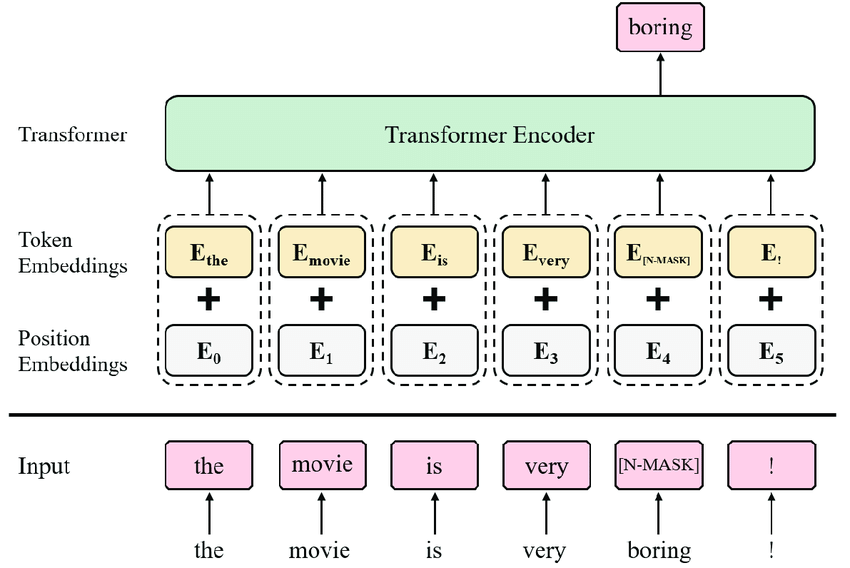
\includegraphics[width=0.95\textwidth]{img/mlm_obj.png}}
    \centering
    \caption{Illustration of MLM objective during the pre-training. Illustration is reprinted from \cite{devlin2018bert}.}
    \label{img:mlmobj}
\end{figure}

We use the default BERT configuration from huggingface to construct the model. A complete list of the hyperparameters can be found on Table \ref{tab:hyp_en} and \ref{tab:hyp_de}.

\begin{table}[]
    \centering
    \begin{tabular}{@{}ccc@{}}
        \toprule
        \textbf{Name}                            & \textbf{Value} & \textbf{Description}                                                                 \\ \midrule
        \textbf{vocab\_size}                     & 30522          & \begin{tabular}[c]{@{}c@{}}Vocabulary size of the\\ BERT model\end{tabular}          \\
        \textbf{hidden\_size}                    & 768            & \begin{tabular}[c]{@{}c@{}}Dimensionality for each\\ of the layers\end{tabular}      \\
        \textbf{num\_hidden\_layers}             & 12             & \begin{tabular}[c]{@{}c@{}}Number of hidden layers\\ in the transformer\end{tabular} \\
        \textbf{num\_attention\_heads}           &
        12                                       &
        \begin{tabular}[c]{@{}c@{}}Number of attention heads for\\ each attention layer\end{tabular}                                                     \\
        \textbf{intermediate\_size}              & 3072           & \begin{tabular}[c]{@{}c@{}}Dimensionality of the\\ feed-forward layer\end{tabular}   \\
        \textbf{hidden\_act}                     & "gelu"         & \begin{tabular}[c]{@{}c@{}}The activation function\\ within the layer\end{tabular}   \\
        \textbf{hidden\_dropout\_prob}           &
        0.1                                      &
        \begin{tabular}[c]{@{}c@{}}The dropout probability\\ for all fully connected layers in\\ the embeddings, encoder,\\ and pooler\end{tabular}      \\
        \textbf{attention\_probs\_dropout\_prob} &
        0.1                                      &
        \begin{tabular}[c]{@{}c@{}}The dropout ratio for the\\ attention probabilities\end{tabular}                                                      \\ \bottomrule
    \end{tabular}
    \caption{Transformer parameter for English based on \texttt{bert-base-uncased}}
    \label{tab:hyp_en}
\end{table}

\begin{table}[]
    \centering
    \begin{tabular}{@{}ccc@{}}
        \toprule
        \textbf{Name}                            & \textbf{Value} & \textbf{Description}                                                                 \\ \midrule
        \textbf{vocab\_size}                     & 31102          & \begin{tabular}[c]{@{}c@{}}Vocabulary size of the\\ BERT model\end{tabular}          \\
        \textbf{hidden\_size}                    & 768            & \begin{tabular}[c]{@{}c@{}}Dimensionality for each\\ of the layers\end{tabular}      \\
        \textbf{num\_hidden\_layers}             & 12             & \begin{tabular}[c]{@{}c@{}}Number of hidden layers\\ in the transformer\end{tabular} \\
        \textbf{num\_attention\_heads}           &
        12                                       &
        \begin{tabular}[c]{@{}c@{}}Number of attention heads for\\ each attention layer\end{tabular}                                                     \\
        \textbf{intermediate\_size}              & 3072           & \begin{tabular}[c]{@{}c@{}}Dimensionality of the\\ feed-forward layer\end{tabular}   \\
        \textbf{hidden\_act}                     & "gelu"         & \begin{tabular}[c]{@{}c@{}}The activation function\\ within the layer\end{tabular}   \\
        \textbf{hidden\_dropout\_prob}           &
        0.1                                      &
        \begin{tabular}[c]{@{}c@{}}The dropout probability\\ for all fully connected layers in\\ the embeddings, encoder,\\ and pooler\end{tabular}      \\
        \textbf{attention\_probs\_dropout\_prob} &
        0.1                                      &
        \begin{tabular}[c]{@{}c@{}}The dropout ratio for the\\ attention probabilities\end{tabular}                                                      \\ \bottomrule
    \end{tabular}
    \caption{Transformer parameter for German based on \texttt{bert-base-german-dbmdz-uncased}.}
    \label{tab:hyp_de}
\end{table}

We train the model until convergence. The definition of convergence in our case for MLM objective is to train the model until the validation loss is no longer improving. Each languages with different number of volumes may end up converging in different steps.

\subsection{Machine Translation}
\subsubsection{Dataset}
In machine translation experiments, there are several scenarios on which we use both WMT and IWSLT dataset. The IWSLT dataset is mainly used for fine-tuning and evaluation of the final model. The WMT, on the other hand, will be combined with IWSLT for training the baseline models. Similar to the language model experiments, we will have three different baselines: IWSLT standalone, IWSLT + WMT (500k), IWSLT + WMT (2 millions). To be more specific, for IWSLT standalone we use the IWSLT dataset for training, evaluation, as well as testing. For the rest of dataset with combination of IWSLT and WMT, we use them for training only while on evaluation and testing we still refer to the IWSLT data alone.

\subsubsection{Model}
We use a sequence-to-sequence architecture described on \cite{vaswani2017attention}. The sequence-to-sequence architecture contains two different components, encoder and decoder. The details and exact figure of this architecture has been described on Chapter 1. The encoder and decoder use the same model and hyperparameters as described in the Section \ref{ssec:langmodel}. The only modification from the original model in language model is in the decoder side. We understand that on the encoder side all the self-attention layer will only refer to the neighbors of theh current layer only for gathering the context. On the other hand, for the decoder, we need further context by including the representation from the eneocder as the extra features. For this reason, an extra layer such as \texttt{cross\_attention} layer is introduced in the decoder and will be trained from scratch for any experiments.

\section{Experiments Results}
This section will discuss the result obtained for machine translation tasks. First, in Section \ref{ssec:adaptcomp}, we conduct the comparative study of using adapters with different scenarios. Second, in Section \ref{ssec:randshuff}, we perform a study by replacing the BERT model with a different BERT version where the weights are shuffled. We continue the study of understanding the adapters behaviour by replacing the pre-trained weights with completely random set of weights and not using the BERT model. Finally, in Section \ref{ssec:randpre}, we perform the experiments to understand the contribution of the total number of sentences used in the pre-training.

\subsection{Adapters Comparison}
\label{ssec:adaptcomp}
\subsubsection{Experiment Setup and Motivation}
We are first trying to understand the contribution of adapters by performing the comparison of models that trained and fine-tuned with different size of datasets. The definition of dataset is the same as have already explained on the previous section. There are three different categories of dataset that is used in two different ways:
\begin{itemize}
    \item Used by baseline model to train the model from scratch
    \item Used for pre-training and later fine-tuned on IWSLT dataset
\end{itemize}

\subsubsection{Experiment Results}
\begin{figure}[h]
    {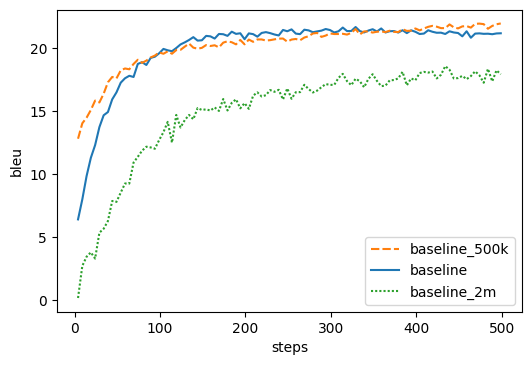
\includegraphics[width=0.95\textwidth]{img/baseline.png}}
    \centering
    \caption{
        Comparison between baseline models trained with different size of datasets. \texttt{baseline} represents the model trained only using IWSLT; \texttt{baseline\_500k} represents the model trained using IWSLT and WMT with total of 500k sentence pairs; \texttt{baseline\_2m} represents the model trained using IWSLT and WMT with total of 2 million sentence pairs.}
    \label{img:basecomp}
\end{figure}

In this section, we compare the result of the baseline models with the models that are fine-tuned with adapters. From Figure \ref{img:basecomp}, adding more data to the baseline models does not necessarily improve the performance. We suspect the models require more time to train to get better performance. There is a clear gap between \texttt{baseline\_2m} and the rest of the baseline models. \texttt{baseline} and \texttt{baseline\_500k} performs really well from the start while \texttt{baseline\_2m} lag behind. We suspect this is the effect of including more sentences from different domains. \texttt{baseline\_500k} is the best mix given the training time constraint. It provides a balance in between not overfitting in the correct domain and not too much data out of the domain. \texttt{baseline\_2m} shows the impact on domain difference. It does not perform well on IWSLT but it is growing and has a chance to improve the performance further. At a later stage, the \texttt{baseline\_2m} output would deserve manual evaluation, because the lower bleu may not necessarily reflect a lower quality, we can see some of the result in Table \ref{tab:qtvout}.

To see the impact of including adapters, we compare the result on different sizes of pre-training used for the base model. The base models are then fine-tuned with the adapters module on the IWSLT data. As we can see from Figure \ref{img:adpcomp}, BERT achieves the best performance from the earlier steps compared to the rest of the pre-training size. In contrast to the baseline models, we see the benefit of adding more sentences to the pre-training. We can see the performance progression between the model that was trained using 500k data has lower performance than the one using 2 million data. On the other hand, models that only use IWSLT as the pre-training data suffers from performance degradation in the middle of the fine-tuning. We observed that this is due to the gradient explosion on the cross-attention layer. The IWSLT model eventually managed to achieve a similar performance to the 500k model in the later steps.
\begin{figure}[h]
    {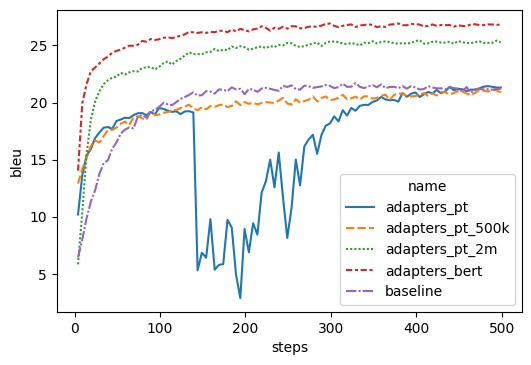
\includegraphics[width=0.95\textwidth]{img/adapterscomparison.png}}
    \centering
    \caption{
        % \XXX{Could you include baseline curve, too? This is rather important for comparison given the lack of the stopping criterion.}
        Comparison between adapters pre-trained with different size of datasets. \texttt{baseline} represents the model trained only using IWSLT; \texttt{adapters\_pt} represents the model pre-trained only using IWSLT; \texttt{adapters\_pt\_500k} represents the model pre-trained using IWSLT and WMT with total of 500k sentence pairs; \texttt{adapters\_pt\_2m} represents the model pre-trained using IWSLT and WMT with total of 2 million sentence pairs; \texttt{adapters\_bert} represents the model that uses BERT weights.}
    \label{img:adpcomp}
\end{figure}

\begin{table*}[]
    \centering
    \begin{tabular}{@{}c@{}}
        \toprule
        \textbf{Random Weights + Adapters}                                                                                                                                                                                                             \\ \midrule
        \begin{tabular}[c]{@{}c@{}}\textbf{input}: wir tanzen im tempel und werden zu gott. \& quot ;\\ \textbf{prediction}: we \& apos ; re going to be able to become god. \& quot ;\end{tabular}                                                    \\ \midrule
        \begin{tabular}[c]{@{}c@{}}\textbf{input}: aber gleichzeitig hatten sie eine klare kenntnis des waldes, \\ die erstaunlich war.\\ \textbf{prediction}: but at the same time, they had a clear of the audience \\ who was amazing.\end{tabular} \\ \midrule
        \begin{tabular}[c]{@{}c@{}}\textbf{input}: es ist so wunderbar. ihr musst es beschutzen. \& quot ;\\ \textbf{prediction}: it \& apos ; s wonderful. you have to protect it. \& quot ;\end{tabular}                                             \\ \bottomrule
    \end{tabular}
    \caption{Prediction results from randomly set pre-trained model fine-tuned with adapters}
    \label{tab:qtrand}
\end{table*}

\subsection{Random and Shuffled Pre-training Weights}
\label{ssec:randshuff}
\subsubsection{Experiment Setup and Motivation}
To show to what extent the Adapter approach benefits from the exact pre-trained weights vs. some of their general distribution properties vs. just the network structure, we conduct experiments where we start by shuffling BERT weights. To perform the experiment, we separate the weights initialization into two approaches: 1) We shuffled the weights from a column perspective. This means in all the weights matrices in the BERT network, we shuffled the weights by preserving columns but shuffling their order. 2) We shuffled the weights from both column and row perspectives.

Furthermore, we also conduct experiments where randomly set weights on all base network layers as the pre-training models. During the fine-tuning, we only update the weights of the adapter and keep the rest of the weights intact.

\subsubsection{Experiment Results}
We can see from Figure \ref{img:shfrndcmp} that the performance of the model that uses random weights as the pre-training model is more stable than the one using shuffled BERT weights. Both of the shuffled BERT models suffer from gradient explosion similar to the IWSLT model we show in the previous section. Although the performance of the random model is still below the baseline model, it is interesting to see that only fine-tuning adapters and the cross-attention layer manage to achieve a reasonable BLEU score, considering that the pre-training models do not contain any meaningful information.
\begin{figure}[h]
    {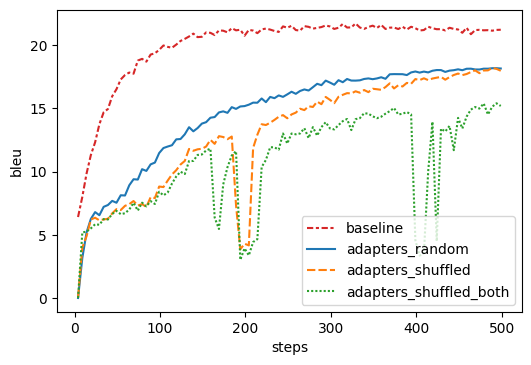
\includegraphics[width=0.95\textwidth]{img/randomshuffled.png}}
    \centering
    \caption{Comparison between adapters using shuffled BERT and random weights as the pre-trained models. \texttt{baseline} represents the model trained only using IWSLT; \texttt{adapters\_random} represents the model pre-trained only using random weights; \texttt{adapters\_shuffled} represents the model pre-trained using column-wise shuffled BERT model; \texttt{adapters\_shuffled\_both} represents the model pre-trained using shuffled BERT model.}
    \label{img:shfrndcmp}
\end{figure}

Since we are relying on the base model with a random set of weights, there is a possibility that our method prone to fallacy that the method only works in a single random seed. To ensure that we perform a robust experiemnt, we repeat the random experiments 10 times with 10 different random seeds $\{42, 438, 87, 555, 492, 252, 843, 561, 734, 194\}$. We can see from the result in Figure \ref{img:rndmseed} that all the random seed performs similarly to one and another.

\begin{figure}[h]
    {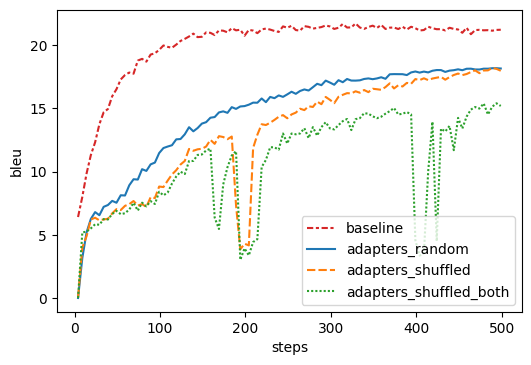
\includegraphics[width=0.95\textwidth]{img/randomshuffled.png}}
    \centering
    \caption{Comparison of different random seed for randomly set weights based models.}
    \label{img:rndmseed}
\end{figure}

\subsection{Random Pretraining vs. Out-of-Domain Data}
\label{ssec:randpre}
\subsubsection{Experiment Setup and Motivation}
In this experiment, we use the same setup as in the Section \ref{ssec:adaptcomp} and \ref{ssec:randshuff}. Specifically, we are interested to investigate the performance of the random weights model compared to the baseline model. We notice that from the previous experiments, we can gain a reasonable score with the random weights model, in this experiment we are conducting further study the performance relative to the baseline where the models were trained using a mix of WMT and IWSLT. The goal of this comparative study is to understand whether we can gain benefit by only fine-tuning a small number of weights (adapters) vs training the whole transformer model with bigger data size.

\subsubsection{Experiment Results}
We further analyze the random weights by comparing the result with the best performing, baseline, and transformer models we pre-trained ourselves. From Figure \ref{img:rndbslcmp}, we can see that the performance of the random model achieves a similar result to the baseline model that uses 2 million training sentence pairs.
This tells us that training the whole models with bigger data does not necessarily improve the model's performance. It may need further tuning to gain benefits of bigger data and bigger model. We can see the result of using random weights as a potential alternative for training the model with small data such as IWSLT.
While the performance is still far from the baseline that is trained using only IWSLT data, this result shows the base model's structure helps the adapter achieve a meaningful performance with very small weights required for the fine-tuning.

We perform a quick check to the output of the model in Table \ref{tab:qtrand}. We can see from the first two lines that the model has difficulty to capture complex phrases. On the first row, the model missed \textbf{tanzen im tempel} which means \textbf{dancing in the temple}. For the second row, the model confuses \textbf{knowledge of the forest} and output \textbf{audience instead}. Furthermore, the model also does not translate the word \textbf{kenntnis} and makes the translation unclear since the object of the sentence is missing. Despite those mistakes, the model still can capture simple sentences as shown on the third row. Another observation that we noticed in the generated output is the tokenization of \texttt{\&quot\;} and \texttt{\&amp\;}. Instead of being treated as a single token, the tokenizer treats the token as three different subword token. We notice that this is due to the inavailability of the aforementioned token in the pre-trained BERT vocabulary.


\begin{figure}[h]
    {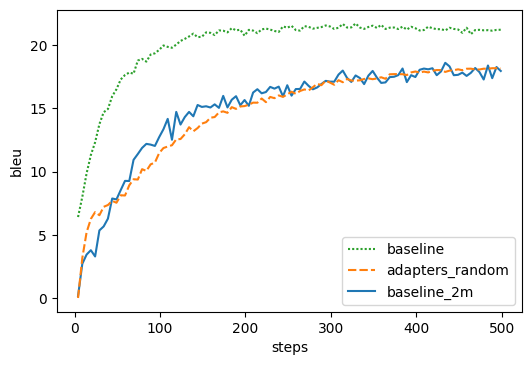
\includegraphics[width=0.95\textwidth]{img/random.png}}
    \centering
    \caption{Comparison between pre-trained random weights and baseline model. \texttt{baseline} represents the model trained only using IWSLT; \texttt{baseline\_2m} represents the baseline model trained with a combination of IWSLT and WMT sentence pairs; \texttt{adapters\_random} represents the model pre-trained only using random weights; \texttt{adapters\_pt\_2m} represents the model pre-trained using IWSLT and WMT with total of 2 million sentence pairs; \texttt{adapters\_bert} represents the model that uses BERT weights}
    \label{img:rndbslcmp}
\end{figure}

\section{Qualitative Comparison}
\begin{sidewaystable*}
    \centering
    \begin{tabular}{|l|l|l|}
        \hline
        \multicolumn{1}{|c|}{\textbf{Baseline IWSLT}}                                                                                                                                                                                                                     &
        \multicolumn{1}{c|}{\textbf{IWSLT + WMT (total 2m)}}                                                                                                                                                                                                              &
        \multicolumn{1}{c|}{\textbf{BERT + Adapters}}                                                                                                                                                                                                                                \\ \hline
        \begin{tabular}[c]{@{}l@{}}\textbf{input}: erinnerst du dich an\\ den patienten\\ mit dem gereizten rachen? \\ \textbf{prediction}: do you remember\\ reading to the patients? on the\end{tabular}                                                                &
        \begin{tabular}[c]{@{}l@{}}\textbf{input}: erinnerst du dich an\\ den patienten\\ mit dem gereizten rachen? \\ \textbf{prediction}: do you remember\\ the patient with the tingling\\ revenge?\end{tabular}                                                       &
        \begin{tabular}[c]{@{}l@{}}\textbf{input}: erinnerst du dich an\\ den patienten\\ mit dem gereizten rachen? \\ \textbf{prediction}: remember the\\ patient with\\ the bruised remorse?\end{tabular}                                                                          \\ \hline
        \begin{tabular}[c]{@{}l@{}}\textbf{input}: großartig, sagte ich.\\ legte auf.\\ \textbf{prediction}: great, i said.\\ got up..\end{tabular}                                                                                                                       &
        \begin{tabular}[c]{@{}l@{}}\textbf{input}: großartig, sagte ich.\\ legte auf.\\ \textbf{prediction}: great, i said.\\ put on..\end{tabular}                                                                                                                       &
        \begin{tabular}[c]{@{}l@{}}\textbf{input}: großartig, sagte ich.\\ legte auf.\\ \textbf{prediction}: great, i said.\\ put it down.\end{tabular}                                                                                                                              \\ \hline
        \begin{tabular}[c]{@{}l@{}}\textbf{input}: - - aber in unserer\\ entdeckung der welt, haben\\ wir alle arten unterschiedlicher\\ methoden.\\ \textbf{prediction}: but in our discovery\\ of the world, we \& apos ;\\ ve got all sorts of different\end{tabular}  &
        \begin{tabular}[c]{@{}l@{}}\textbf{input}: - - aber in unserer\\ entdeckung der welt, haben\\ wir alle arten unterschiedlicher\\ methoden.\\ \textbf{prediction}: - - but in our discovery\\ of the world, we have\\ all kinds of different methods.\end{tabular} &
        \begin{tabular}[c]{@{}l@{}}\textbf{input}: - - aber in unserer\\ entdeckung der welt, haben\\ wir alle arten unterschiedlicher\\ methoden.\\ \textbf{prediction}: but in our discovery\\ of the world, we have\\ all sorts of different ways of doing\\ things.\end{tabular} \\ \hline
    \end{tabular}
    \caption{Prediction results from 1) Baseline model trained with only IWSLT data; 2) Pre-trained model with adapters where we pre-train the model with IWSLT and WMT with a total of 2 million pre-training data; 3) BERT with adapters.}
    \label{tab:qtvout}
\end{sidewaystable*}
We perform a sanity check to compare the generated results on some of our models. This sanity check is to check the errors produced by the models on different techniques.
From Table \ref{tab:qtvout}, we can see for the first example none of the models managed to generate the correct result. However, BERT + adapters and 2 million pre-trained base models manage to generate the proper context where the result is still discussing \textbf{the patient}. The wrong part is when the model generates an incorrect translation regarding the patient's disease. The second example shows that the BERT + adapters create the correct and better output than the other models. The final example shows that BERT + adapters generate an interesting output where it manages to remove unimportant characters such as \texttt{--} and produce readable output. There may be a slightly different opinion on this example as the 2 million pre-trained base model generate a more concise output.

% Target: 35 pages
% Current: 3

\chapter{Adapters Effectiveness in Machine Translation}
\label{chap:adaptefct}
We continue the study from the previous chapter to understand more about the relation between adapters and pre-trained models. Similar to the previous chapter, we use BERT and its variants as the pre-trained models and fine-tune them with adapters. This study aims to evaluate the combination of adapters and BERT in machine translation and study the effectiveness of adapters by putting them only in the encoder or the decoder. We also experiment with down-scaling the pre-trained model size and try to recover the performance of the full-sized model. We separate the experiments into three different areas:
\begin{itemize}
    \item Use BERT weights\footnote{We use publicly available BERT model from Huggingface hub \url{https://huggingface.co}} as the pre-trained weights and investigate the importance of adapters in encoder or decoder.
    \item Use BERT weights and investigate their importance compared to random weights in the encoder or decoder while fine-tuning with adapters.
    \item Down-scaling BERT weights by either zeroing out half of BERT's weights (\texttt{zbert}) or completely removing them from the weight matrices, squashing the matrices (\texttt{zsbert}). We use the down-scaling technique to understand whether we can use adapters to recover the performance of the original BERT (without adapters) while using fewer parameters.
\end{itemize}

\section{Fixed Variable Parameters of Experients}
\subsection{Framework}
% \begin{table}[t]
%     \centering
%     \begin{tabular}{@{}cc@{}}
%         \toprule
%         \textbf{Name}            & \textbf{Value}        \\ \midrule
%         \textbf{Batch size}      & 64                    \\
%         \textbf{Learning rate}   & 0.0005                \\
%         \textbf{Vocabulary size} & 31102 (de), 30522(en) \\ \bottomrule
%     \end{tabular}
%     \caption{Fixed hyperparameters throughout the experiments}
%     \label{tab:hyp_invest}
% \end{table}

As we mentioned at the beginning of the chapter, we have several scenarios we use to conduct the experiments. We start by describing the variables that we fixed throughout the experiments. As we have mentioned in \cref{chap:03}, we use Huggingface as our main framework with added modifications for adapters. Contrary to \cref{chap:adaptmt}, we do not investigate language models that we train ourselves, but instead, we focus only on the BERT language model.

The model and hyperparameters that we use throughout the experiment remain the same as described in \cref{chap:adaptmt}. We use transformer model with seq2seq architecture and the BERT-based hyperparameter configuration to initialize both the encoder and the decoder.

\subsection{Dataset}
As mentioned in the previous section, our focus in this chapter is on machine translation. We use IWSLT dataset to perform the fine-tuning as well as the evaluation for the models.

\section{Original BERT}
\subsection{Size of Adapters}
\subsubsection{Experiment Setup and Motivation}
\paragraph{}
In these experiments, we freeze both the encoder and decoder and modify the reduction ratio parameter in the adapters. The adapter serves as a bottleneck layer with two dense layers and a non-linear function between them. The reduction ratio is defined as the fraction of the original representation dimension divided by the adapter vector size. For instance, if we use 16 as the reduction ratio, we reduce the original layers by 16 with the first dense layer and then scale it back to the original size with the second dense layer.

We try out various sizes of reduction ratios to compare the results. This reduction aims to see whether we can further benefit from enlarging the adapters' bottleneck size. We use 16, 8, 4, 2, and 1 as the ratio values for this experiment. We compare the results with the baseline BERT that we fine-tuned by only training the cross-attention and output layers. We will refer to this baseline as \texttt{baseline\_bert} for the entirety of this chapter.

\subsubsection{Experiment Results}
In this section, we compare the results of the \texttt{baseline\_bert} with BERT models that are fine-tuned with adapters in different reduction ratios. We are fine-tuning the cross-attention and output layers for the \texttt{baseline\_bert} model and freeze the rest of the model. We can see in \cref{img:adapt_bert_ratio} that even the smallest model (\texttt{adapt\_bert\_reduc\_16}) can already outperform the baseline by around 2 BLEU points. This shows that the adapters can help improve the model's performance by adding only a small number of weights during the fine-tuning.

\begin{figure}[]
    {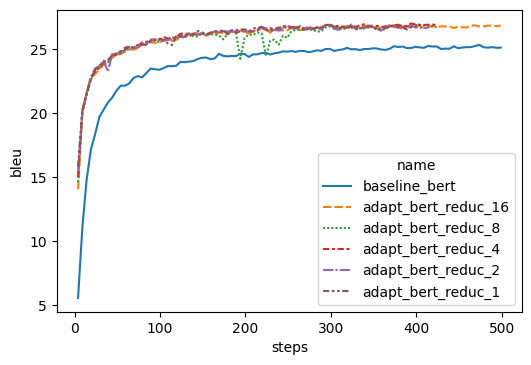
\includegraphics[width=0.85\textwidth]{img/adapter_bert_baseline_adapters.png}}
    \centering
    \caption{Comparison between baseline BERT model and adapters model with different ratio (16, 8, 4, 2, 1).}
    \label{img:adapt_bert_ratio}
\end{figure}

Despite better performance than the baseline model, the difference between the ratios is minimal. It suggests that there is not much benefit in expanding the size of adapters for the normal size BERT. It is possible that it is no longer trivial to simply append larger-size adapters for fine-tuning the model and getting better performance. Further changes may be required to handle the different nature of BERT's output as it is naturally different from the common auto-regressive machine translation objective. Furthermore, we recall that we also have problems where the models struggle in generating good translations when the input contains an unavailable token such as \texttt{\&quot\;}.

\subsection{Position of Adapters (Encoder vs Decoder)}
\label{sec:posada}
\subsubsection{Experiment Setup and Motivation}
We would like to see the importance of adapters when they are put in different places. Since we are working with seq2seq architecture in this work, we would like to see whether only incorporating adapters on either the encoder or the decoder can already be beneficial and reduce the number of parameters added to the model.

\subsubsection{Experiment Result}
\begin{figure}[]
    {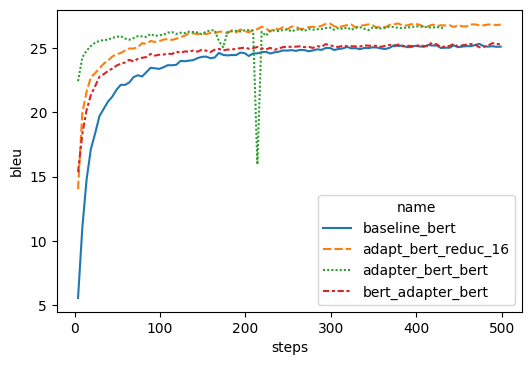
\includegraphics[width=0.85\textwidth]{img/bert_pos.png}}
    \centering
    \caption[Results of ablation study for adapters in the encoder or the decoder.]{Comparison between baseline BERT model and adapters model where the adapters are placed in three different setups: 1) Adapters in both encoder and decoder (\texttt{adapt\_bert\_reduc\_16}); 2) Adapters only in encoder (\texttt{adapter\_bert\_bert}); 3) Adapters only in decoder (\texttt{bert\_adapter\_bert}).}
    \label{img:adapt_bert_pos}
\end{figure}
We see in \cref{img:adapt_bert_pos} that adding adapters just in the encoder brings an improvement and outperforms the baseline. Adapters only in the encoder train the fastest at the beginning, and their final performance is almost the same as if we added the adapters on both sides. For the decoder, on the other hand, we can see that aside from a more promising start, there is no benefit as there is no improvement in terms of late BLEU scores compared to the baseline. With this finding, we can reduce the cost of fine-tuning further by half when we do not include the adapters on the decoder.
% Adding the adapters on the encoder and fine-tuning it is more cost-effective than the decoder. With this finding, we can reduce the cost of fine-tuning by half when we do not include the adapters on the decoder.

\subsection{True BERT in Encoder vs Decoder}
\label{sec:pospre}
\subsubsection{Experiment Setup and Motivation}
This section investigates the importance of pre-trained BERT in the encoder or the decoder when the adapters are used for fine-tuning the models.
% In addition to that, we also expand the experiment further by understanding the correlation of adding adapters on top of the randomly set weights.

% We start by describing the setup in this experiment. 
The previous chapter introduced an experiment where we instantiate the base transformer model with only random fixed weights. We are then fine-tuning the base transformer model by only updating the cross-attention, adapters, and output layers. In this setup, we are doing experiments in a similar concept. We use random (fixed) weights instead of the original pre-trained BERT weights in the encoder or the decoder. We thus have a seq2seq model with the random weights encoder followed by the BERT decoder and vice versa. In the fine-tuning stage, we update the adapters in the encoder and decoder, the cross-attention (or cross-attention layer only in our baseline models), and the output layers.

The purposes of the experiments are:
\begin{itemize}
    \item We want to understand further the importance of the pre-training model when fine-tuning with adapters. By initializing the models with BERT only in one component, we can see whether it is necessary to use BERT on both components when adapters are incorporated.
    \item We want to understand the capability of adapters when either one of the components does not contain useful information (relative to BERT). We would like to see whether the adapters can recover or even outperform some of the performance that we have already gathered from the previous chapters and sections.
\end{itemize}

\subsubsection{Experiment Results}
This section compares models that use adapters in either or both the encoder and decoder while only initializing one of these components with pre-trained BERT and the other one with (fixed) random weights.

\paragraph{Randomly Set Weights on Encoder}
In this part of the section, we want to answer the main question: ``To what extent can the adapters restore the missing gap when the encoder does not contain useful information (relative to BERT)?''

We can see from \cref{img:adapt_bert_randenc} that when adapters are used in both components to a model with random encoder weights (\texttt{adapter\_randenc\_adapter\_bert}), we get to almost 20 BLEU points. This is relatively higher than the other two setups: adapters only in the encoder (\texttt{adapter\_randenc\_bert}) and only in the decoder (\texttt{randenc\_adapter\_bert}). However, compared to the baseline, we are missing 4 BLEU points when we set the encoder with completely random weights. This means that the base encoder model did contain relatively essential information that the adapters can not simply restore during the fine-tuning.

\begin{figure}[t]
    {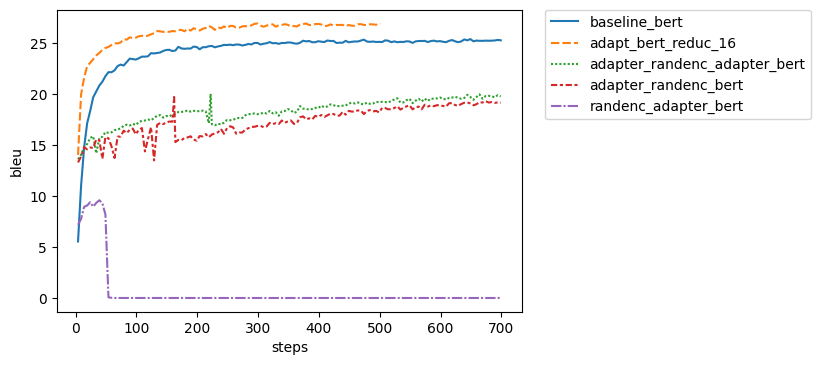
\includegraphics[width=0.85\textwidth]{img/adapter_bert_randenc.png}}
    \centering
    \caption[Random + BERT: Comparison for model with adapters in the decoder and the encoder is initalized with random weights.]{Random + BERT: Comparison between baseline BERT model and adapters model where the adapters are placed in three different setups: 1) Adapters in both encoder and decoder (\texttt{adapt\_bert\_reduc\_16}); 2) Adapters only in encoder (\texttt{adapter\_bert\_bert}); 3) Adapters only in decoder (\texttt{bert\_adapter\_bert}) and the decoder is initialized with BERT while the encoder is initialized with random numbers.}
    \label{img:adapt_bert_randenc}
\end{figure}

% We further focus on the adapters' performance compared to the baseline model that is only fine-tuned on the cross-attention layer to see whether fine-tuning the cross-attention is already enough or if there is any benefit in adding adapters. We can see that the model that only fine-tuning the cross-attention layer (\texttt{baseline\_bert}) can not learn at all, while the adapters can perform significantly better. This marks the capability of the adapter when faced with a randomly set encoder.

When the adapters are removed from the decoder (\texttt{adapter\_randenc\_bert}), we see a degradation in performance about 1 BLEU point compared to the model that uses adapters on both side (\texttt{adapter\_randenc\_adapter\_bert}). However, when the adapters are removed from the encoder (\texttt{randenc\_adapter\_bert}), the performance is completely depleted to zero during the training. We also see the same behaviour in the next section when the weights on the decoder are set randomly. This tells us that it is not trivial to simply fine-tune the cross-attention without further modifying the encoder's parameters when the parameters on the encoder are completely random.

\paragraph{Randomly Set Weights on Decoder}
Similar to the previous section, the main question in this experiment is, ``To what extent can the adapters restore the performance when the decoder does not contain useful information (relative to BERT)?''

In contrast to when the randomly set weights are on the encoder side, we can see from \cref{img:adapt_bert_randdec} that fixing a random decoder leads to performance comparable to the one we have on \texttt{bert\_baseline}. This tells us that the pre-trained weights in the encoder are more important than in the decoder when we have adapters on both sides. However, when removing the adapters on the encoder, we see similar performance as in the previous section, where the performance drops to zero in the middle of training. This further strengthens our argument that adapters are necessary to adjust the weights in the model so that the cross-attention layer can work properly.

\begin{figure}[h]
    {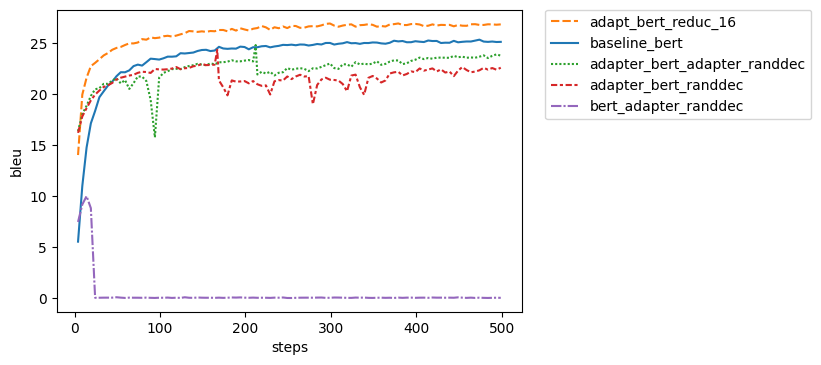
\includegraphics[width=0.85\textwidth]{img/adapter_bert_randdec.png}}
    \centering
    \caption[BERT + Random: Comparison for model with adapters in the decoder and the decoder is initalized with random weights]{BERT + Random: Comparison between baseline BERT model and adapters model where the adapters are placed in three different setups: 1) Adapters in both encoder and decoder (\texttt{adapt\_bert\_reduc\_16}); 2) Adapters only in encoder (\texttt{adapter\_bert\_bert}); 3) Adapters only in decoder (\texttt{bert\_adapter\_bert}) and the encoder is initialized with BERT while the decoder is initialized with random numbers.}
    \label{img:adapt_bert_randdec}
\end{figure}

On the other hand, when we remove the adapters from the decoder side, we can see that the performance is not as bad as when the adapters are removed from the encoder, but we still see a reduction in performance. We see a reduction around less than 1 BLEU point when the model reaches 400k steps in the training stage. It is possible that even with random weights on the decoder side, the adapters help the cross-attention layers produce a good vector representation with meaningful features for the decoder to generate reasonable translation outputs.

\section{BERT Size Reduction}
\subsection{Zeroing Columns}
\subsubsection{Experiment Setup and Motivation}
In this experiment, we will focus on the soft reduction of BERT weights by zeroing the weight matrices on every even column and row indices within the transformer body as well as in the embedding. We load the pre-trained BERT weights, manually edit them and then continue the experiments by fine-tuning the cross-attention, adapters, and output layers. We refer to this setup as \texttt{zbert} for the rest of this chapter.

Besides removing the columns, we also perform experiments where we put the adapters either on the encoder or the decoder. This particular experiment aims to understand the model's behaviour when the pre-trained BERT is replaced with this particular setup.

\subsubsection{Comparison with BERT Baseline (Full BERT Fine-tuning)}
We first compare the \texttt{zbert} model without adapters and only fine-tune the cross-attention and output layers. We use \texttt{zbert} weights on both the encoder and decoder so that it is comparable to the model that uses full-weight BERT. We use the full-weight BERT as the baseline in this experiment.

\begin{figure}[]
    {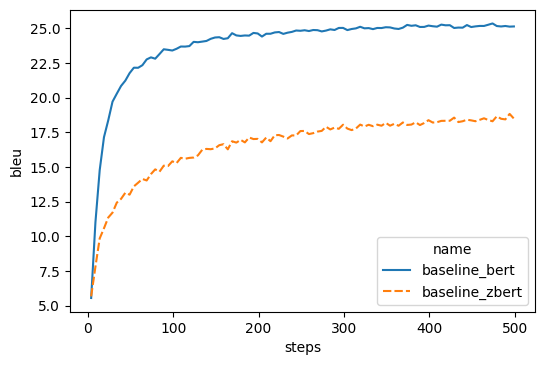
\includegraphics[width=0.85\textwidth]{img/baseline_zbert.png}}
    \centering
    \caption{Comparison between baseline BERT model and baseline \texttt{zbert} models.}
    \label{img:baseline_zbert}
\end{figure}

\begin{figure}[]
    {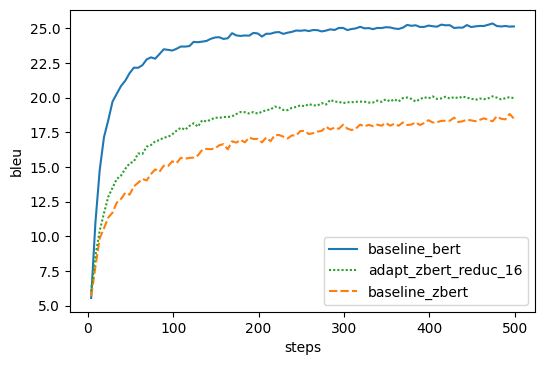
\includegraphics[width=0.85\textwidth]{img/adapter_zbert.png}}
    \centering
    \caption{Comparison between baseline BERT model, baseline \texttt{zbert} and adapters \texttt{zbert} models.}
    \label{img:adapter_zbert}
\end{figure}

We can see in \cref{img:baseline_zbert} that we are losing performance of about 4 BLEU points. This is significant as we lose essential features from the original BERT model. To see whether we can recover some of the performance with adapters, we continue our experiment by fine-tuning the \texttt{zbert} model that is instantiated on both encoder and decoder sides with adapters. We can see from \cref{img:adapter_zbert} that we only managed to recover 1 BLEU point with a reduction ratio of 16.

\begin{figure}[]
    {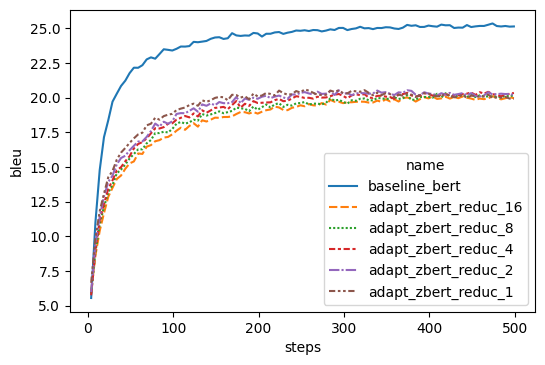
\includegraphics[width=0.85\textwidth]{img/adapter_zbert_ratio.png}}
    \centering
    \caption{Comparison between baseline BERT model and different reduction ratio of \texttt{zbert} models.}
    \label{img:adapter_zbert_ratio}
\end{figure}

From \cref{img:adapter_zbert_ratio}, when we increase the size of the reduction ratio, initially, we can see some improvement in the BLEU score compared to the higher ratio. However, they eventually converge to a similar performance by the end of training with no significant difference between different ratios. From this result, we can understand that depending on the base pre-trained model, adapters still have a limitation in achieving certain performance.

\paragraph{Adapters Position}
In this section, we aim to understand whether the position of both adapters and the pre-trained models affect the model's performance, similar to what we have seen in \cref{sec:posada}. We use a similar setup as in the previous section, with the exception that we use \texttt{zbert} as the pre-trained model instead of the original BERT model.

\begin{figure}[h]
    {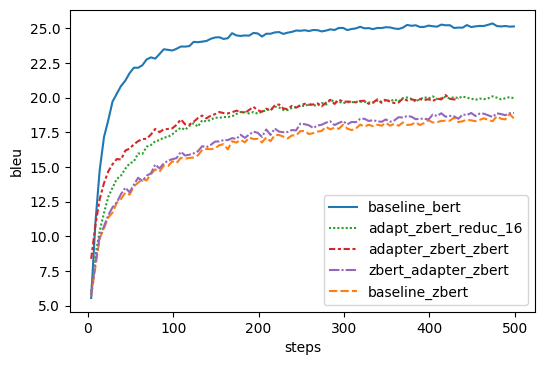
\includegraphics[width=0.85\textwidth]{img/zbert_pos.png}}
    \centering
    \caption[Comparison between baseline BERT and \texttt{zbert} models.]{Comparison between baseline BERT model, baseline \texttt{zbert} model, adapters in both encoder and decoder of \texttt{zbert} model (\texttt{adapt\_zbert\_reduc\_16}), adapters only in encoder of \texttt{zbert} model (\texttt{adapter\_zbert\_zbert}), and adapters only in decoder of \texttt{zbert} model (\texttt{zbert\_adapter\_zbert}).}
    \label{img:zbert_pos}
\end{figure}

We can see from \cref{img:zbert_pos} that when we include adapters on both the encoder and decoder, we can outperform the baseline \texttt{zbert} in around 2 BLEU points. This shows that, similar to the models that use BERT as the pre-trained model, the adapters can help to improve the performance further, even though some of the information is already missing in the base model.

Furthermore, we can also see that, similar to the BERT model experiments, fine-tuning with adapters only on the encoder side (\texttt{adapter\_zbert\_zbert}) performs much better than on the decoder side (\texttt{zbert\_adapter\_zbert}). Other than that, we can also see that incorporating adapters only on the encoder side helps the model achieve better performance faster than using adapters on both sides. This further supports our hypothesis that updating the representation on the encoder side is more beneficial. Additionally, we can also see the same behaviour as the original pre-trained BERT that \texttt{zbert\_adapter\_zbert} performance is close to the baseline model (\texttt{baseline\_zbert}), where we are only fine-tuning the cross-attention and output layers. This could mean that fine-tuning the decoder may not be enough to achieve better performance when the representation from the source side is unchanged.

\subsection{Model Down-Scaling}
\subsubsection{Experiment Setup and Motivation}
This experiment is the follow-up from \texttt{zbert}, where we zeroed out half of the elements in the matrices. More specifically, we are completely removing those elements from the matrix instead of just zeroing out the elements. The way we do this is similar to the one we do on \texttt{zsbert}. We remove the matrix elements on every even column and row in the transformer body and the embedding. We again do the weights processing offline before using it as the pre-trained model. For the rest of this writing, we refer to this setup as \texttt{zsbert}.

Furthermore, we also follow a similar setup as in \cref{sec:posada} where we experiment with the position of the adapters. The goal of this experiment is to understand the behaviour of this model compared to the baseline as well as \texttt{zbert}.

\subsubsection{Comparison with BERT Baseline and \texttt{zbert}}
\label{sec:compbasezbertzsbert}

\begin{figure}[t]
    {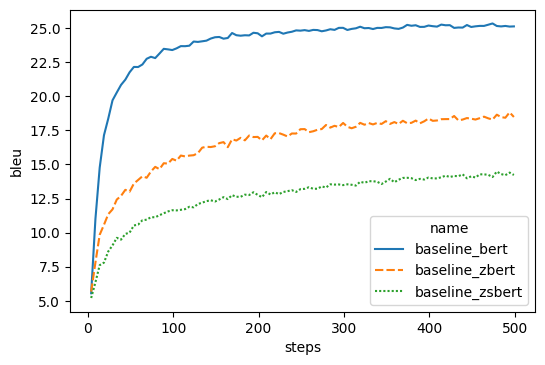
\includegraphics[width=0.85\textwidth]{img/baseline_zsbert.png}}
    \centering
    \caption{Comparison between baseline BERT model and baseline \texttt{zsbert} model.}
    \label{img:baseline_zsbert}
\end{figure}

\begin{figure}[]
    {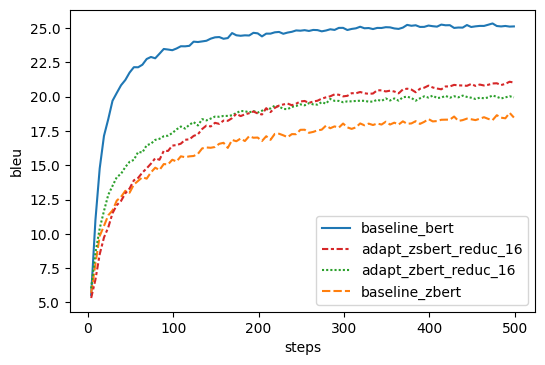
\includegraphics[width=0.85\textwidth]{img/adapter_zsbert.png}}
    \centering
    \caption{Comparison between baseline BERT model, baseline \texttt{zbert}, baseline \texttt{zsbert} and adapters \texttt{zsbert} models.}
    \label{img:adapter_zsbert}
\end{figure}


We begin by comparing \texttt{zsbert} with the BERT baseline. We see in \cref{img:baseline_zsbert} that the performance degrades by more than 10 BLEU points. This is also significantly worse than \texttt{zbert}, where we only lose 7.5 BLEU points. Our initial hypothesis was that \texttt{zsbert}'s performance should be comparable to \texttt{zbert} as we are fundamentally performing the same reduction technique. After some investigation, we realized that removing the weights from the network and zeroing out the matrices are not directly comparable because we also need to consider the computation of layer normalization, which highly depends on the matrix dimension. We found this discrepancy by performing a manual evaluation where we used an arbitrary vector as the input to the network and monitored the output in each of the network layers. We found a slight difference in the layer's output between the zeroed and completely removed weights. Even though the difference is minimal, the output discrepancy gets propagated to the top layers, causing the final network output to differ significantly.

Next, we study the interplay of model down-scaling and adapters. We can see in \cref{img:adapter_zsbert} that \texttt{zsbert} with a 16 ratio adapters manages to improve the performance up to 6 BLEU points compared to \texttt{zbert} without adapters. This shows that adapters can still improve the model's performance even when some weights are missing. Furthermore, despite still showing difficulties in reaching the baseline performance, \cref{img:adapter_zsbert_ratio} shows that we can still improve the model's performance by reducing the adapters reduction ratio.
We can see that the model with the lowest reduction ratio (1) manages to close the performance gap significantly with the baseline model. This is one of our prominent results because we can see from \cref{tab:numvars} that the total number of weights (including adapters) required to fine-tune the model is significantly lower than the original BERT model.
% We also notice a leap in final performance when we compare the adapter model with an equal reduction ratio (16) between \texttt{zbert} and \texttt{zsbert}. We can see that initially \texttt{zsbert} performs worse than \texttt{zbert}. After some steps, we can see the performance in \texttt{zbert} starting to stall but not in \texttt{zsbert}. We hypothesize that this relates to a similar reason that we stated in the original BERT model, where we could not see any improvement when increasing the reduction ratio. It is possible that when we reduce the size of the original pre-trained model, the adapters manage to adjust the flow of information within the network and better replace the missing information with new knowledge that is more important for solving the task.

\begin{figure}[]
    {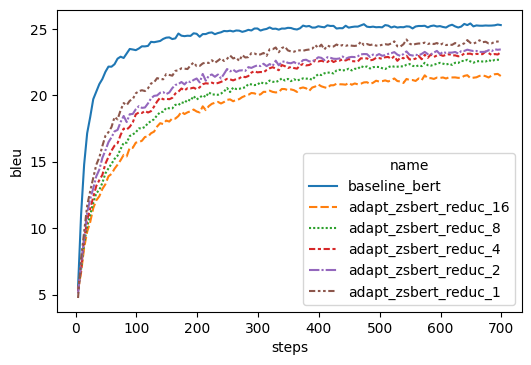
\includegraphics[width=0.85\textwidth]{img/adapter_zsbert_ratio.png}}
    \centering
    \caption{Comparison between baseline BERT model and different reduction ratio of \texttt{zsbert} models.}
    \label{img:adapter_zsbert_ratio}
\end{figure}


\begin{table*}[]
    \centering
    \begin{tabular}{@{}|l|r|r|r|r|@{}}
        \toprule
        \multicolumn{1}{|c|}{\textbf{Name}}                                                              &
        \multicolumn{1}{c|}{\textbf{\begin{tabular}[c]{@{}c@{}}\# Trainable\\  Variables\end{tabular}}}  &
        \multicolumn{1}{c|}{\textbf{\begin{tabular}[c]{@{}c@{}}\# Untrainable\\ Variables\end{tabular}}} &
        \multicolumn{1}{c|}{\textbf{\begin{tabular}[c]{@{}c@{}}\# Total\\ Variables\end{tabular}}}       &
        \multicolumn{1}{c|}{\textbf{\begin{tabular}[c]{@{}c@{}}Percentage\\ Trainable\end{tabular}}}                                                      \\ \midrule
        \textbf{Ratio 16}                                                                                & 7.736.826  & 95.143.296 & 102.880.122 & 7.5\%  \\
        \textbf{Ratio 8}                                                                                 & 8.179.770  & 95.143.296 & 103.323.066 & 7.9\%  \\
        \textbf{Ratio 4}                                                                                 & 9.065.658  & 95.143.296 & 104.208.954 & 8.7\%  \\
        \textbf{Ratio 2}                                                                                 & 10.837.434 & 95.143.296 & 105.980.730 & 10.2\% \\
        \textbf{Ratio 1}                                                                                 & 14.380.986 & 95.143.296 & 109.524.282 & 13.1\% \\ \bottomrule
    \end{tabular}
    \caption{Total trainable variables in \texttt{zsbert} with adapters on different ratio vs normal BERT model}
    \label{tab:numvars}
\end{table*}

\subsubsection{Adapters Position}

\begin{figure}[h]
    {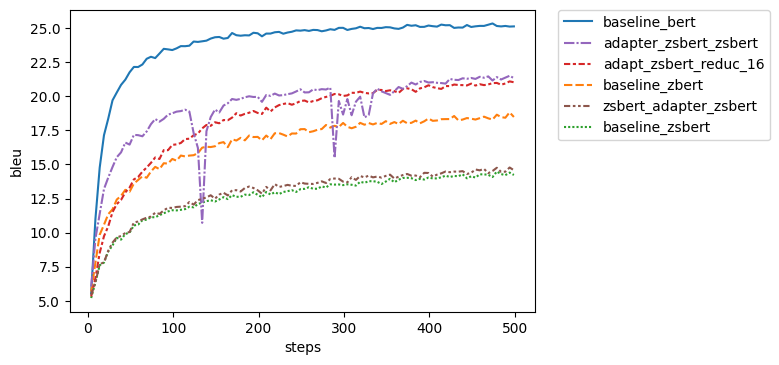
\includegraphics[width=0.85\textwidth]{img/zsbert_pos.png}}
    \centering
    \caption[Comparison between baseline BERT and \texttt{zsbert} models.]{Comparison between baseline BERT model, baseline \texttt{zsbert} model, adapters in both encoder and decoder of \texttt{zsbert} model (\texttt{adapt\_zsbert\_reduc\_16}), adapters only in encoder of \texttt{zsbert} model (\texttt{adapter\_zsbert\_zsbert}), and adapters only in decoder of \texttt{zsbert} model (\texttt{zsbert\_adapter\_zsbert}).}
    \label{img:zsbert_pos}
\end{figure}

From \cref{img:zsbert_pos}, similar to the \texttt{zbert} experiments, we can see similar behaviour where models fine-tuned with adapters outperform the baseline \texttt{zsbert} and \texttt{zbert} models. However, compared to \texttt{zbert} experiments, we notice a bigger improvement in \texttt{zsbert}'s final performance. In \texttt{zbert}, the difference between baseline and adapters is within 5 BLEU points. On the other hand, in \texttt{zsbert}, we see the improvement is within 8 BLEU points. This result is particularly interesting for us as we expect the difference to be similar to \texttt{zbert}. We recall from \ref{sec:compbasezbertzsbert} that this is due to the numerical error from the layer normalization, i.e. a difference in constant used to perform vector normalization in the layer normalization. In other words, we observed a worse performance in \texttt{zbert} than we got for \texttt{zsbert} with adapters.

We deep-dive further in \cref{img:zbert_vs_zsbert} to show the comparison between adapters in \texttt{zbert} and \texttt{zsbert}. We use a reduction ratio of 16 to compare the adapter's performance between these two setups. We notice a leap in the final performance when we compare the adapter model with an equal reduction ratio (16) between \texttt{zbert} and \texttt{zsbert}. We can see that initially \texttt{zsbert} performs worse than \texttt{zbert}. After some steps, we can see the performance in \texttt{zbert} starting to stall but not in \texttt{zsbert}. We hypothesize that this relates to a similar reason we stated in the original BERT model, where we could not see any improvement when increasing the reduction ratio. It is possible that when we reduce the original pre-trained model's size, the adapters adjust the flow of information within the network and better replace the missing information with new knowledge that is more important for solving the task. Another possibility is simply because \texttt{zbert} is a "heavier model" than \texttt{zsbert} as it contains more parameters and thus has a harder time for the adapters to recover.

\begin{figure}[t]
    {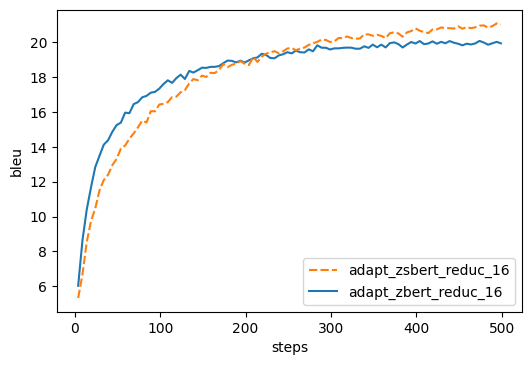
\includegraphics[width=0.85\textwidth]{img/zbert_vs_zsbert.png}}
    \centering
    \caption{Comparison adapters performance in \texttt{zsbert} and \texttt{zbert}. Both are using reduction ratio 16 and the adapters are placed on encoder and decoder.}
    \label{img:zbert_vs_zsbert}
\end{figure}

We see a similar behaviour as in \texttt{zbert} experiments concerning the position of the adapters. In \cref{img:zsbert_pos}, the benefit of incorporating adapters on the encoder side is apparent and outperforms the decoder counterpart. We can also see a similar behaviour where the model's performance with adapters on the encoder eventually outperforms the model with adapters on both sides. Furthermore, we also see a similar behaviour as in \texttt{zbert} for models with adapters in the decoder only where the performance is very close to the baseline and not improving as much as on the encoder side. We hypothesize that the same reason as we have stated in \texttt{zbert} could apply in \texttt{zsbert} as well. Essentially, we need to modify the representation on the encoder side in order to achieve better performance.

\chapter*{Conclusion}
\addcontentsline{toc}{chapter}{Conclusion}


%%% Bibliography
%%% Bibliography (literature used as a source)
%%%
%%% We employ bibTeX to construct the bibliography. It processes
%%% citations in the text (e.g., the \cite{...} macro) and looks up
%%% relevant entries in the bibliography.bib file.
%%%
%%% The \bibliographystyle command selects, which style will be used
%%% for references from the text. The argument in curly brackets is
%%% the name of the corresponding style file (*.bst). Both styles
%%% mentioned in this template are included in LaTeX distributions.

\bibliographystyle{plainnat}    %% Author (year)
% \bibliographystyle{unsrt}     %% [number]

\renewcommand{\bibname}{Bibliography}

%%% Generate the bibliography. Beware that if you cited no works,
%%% the empty list will be omitted completely.

\bibliography{bibliography}

%%% If case you prefer to write the bibliography manually (without bibTeX),
%%% you can use the following. Please follow the ISO 690 standard and
%%% citation conventions of your field of research.

% \begin{thebibliography}{99}
%
% \bibitem{lamport94}
%   {\sc Lamport,} Leslie.
%   \emph{\LaTeX: A Document Preparation System}.
%   2nd edition.
%   Massachusetts: Addison Wesley, 1994.
%   ISBN 0-201-52983-1.
%
% \end{thebibliography}


%%% Figures used in the thesis (consider if this is needed)
\listoffigures

%%% Tables used in the thesis (consider if this is needed)
%%% In mathematical theses, it could be better to move the list of tables to the beginning of the thesis.
\listoftables

%%% Abbreviations used in the thesis, if any, including their explanation
%%% In mathematical theses, it could be better to move the list of abbreviations to the beginning of the thesis.
\chapwithtoc{List of Abbreviations}

%%% Attachments to the master thesis, if any. Each attachment must be
%%% referred to at least once from the text of the thesis. Attachments
%%% are numbered.
%%%
%%% The printed version should preferably contain attachments, which can be
%%% read (additional tables and charts, supplementary text, examples of
%%% program output, etc.). The electronic version is more suited for attachments
%%% which will likely be used in an electronic form rather than read (program
%%% source code, data files, interactive charts, etc.). Electronic attachments
%%% should be uploaded to SIS and optionally also included in the thesis on a~CD/DVD.
%%% Allowed file formats are specified in provision of the rector no. 72/2017.
\appendix
\chapter{Attachments}

\section{First Attachment}

\openright
\end{document}
